\section{The Fall from the Primordial State}

\begin{wrapfigure}{rt}{.3\textwidth}
 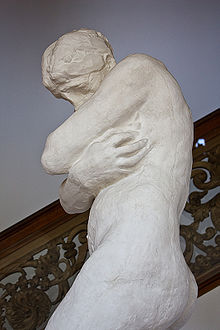
\includegraphics[scale=1.5]{a20110111TheFallfromthePrimordialState-img001.jpg}
\end{wrapfigure}

Let us be clear. The \textbf{Primordial State} is not a ``state of nature" as in Rousseau, but rather of supernature. But if in the Primordial State man lives in harmony with nature and the divine, with a direct awareness of God in his psyche as his life force, and with bonds of loyalty to his family and nation, then what would account for a change in consciousness? Table~\ref{tab:FallPrimordialState1} shows the effects of the Fall in the \emph{Genesis} account, and the corresponding condition that was affected.

\begin{table}[h]
\centering\small
\begin{tabular}{cc}\toprule
\textbf{Effect of Fall} &
\textbf{Consciousness before fall}\\\toprule
Toil &
Concentration without effort\\\midrule
Suffering &
Natural joy\\\midrule
Death &
Transformation\\\bottomrule
\end{tabular}
\caption{The effect of the Fall according to Genesis book.}
\label{tab:FallPrimordialState1}
\end{table}

\paragraph{Effects of the Fall}
The point to keep in mind is that the Fall is an event in consciousness; it is necessary to meditate on the symbols of the fall, and the description of the states, to fully understand.

\begin{description}
\item[Toil ]

Everyone has had the experience of being totally absorbed in an activity, to the extent that time seems to stand still. One feels energized and does not tire. Similarly, composers and poets have often described moments of inspiration, and the poem or symphony seems to write itself. This state of ``concentration without effort" is comparable to the Taoist ideal of \emph{wei-wu-wei}, or doing-nondoing. After the fall, concentration becomes difficult and labored; one becomes restless and bored; activities begin to feel like toil. 

\item[Suffering ]

Man lived in a state of natural joy. The sensory experience of the natural world was vivid and pleasurable; it did not require a special trip to a resort. Man was in communication with the gods and angels, was aware of the presence of his ancestors. He lived in peace with his nation and leaders without private concerns. This was replaced with feelings of resentment and ambition. This led to frustration, anxiety, shame, guilt, and fear. Man became alienated from nature, from the divine, from his nation, and leaders. 

\item[Death ]

Death was understood as a natural process and it represented a transformation. A man was prepared for his death by understanding the post-mortem states of being. He was aware of his ancestors and felt his immortality in his descendants. After the fall, man lost direct awareness of the divine, of his ancestors, of post-mortem states, of his own true Self. Death became something to fear, something that signified destruction rather than transformation. 

\end{description}
\paragraph{Perversion of Soul Life}
The psyche, or soul, which had been a pure reflector of both nature and the divine, becomes obsessed with the effects of the fall. The consequence is that the formerly direct intuitive awareness of nature, the divine, and nation becomes occluded. The true Self is decentered and a false self is established. \textbf{Julian Jaynes} describes the characteristics of this state. [See Note.]

\begin{description}
\item[Spatialization ]

A mind-space model of consciousness is invented. 

\item[Excerption ]

Consciousness is focused on just a part of experience. The vividness of the Primordial State is lost. 

\item[Analog I ]

A model of one's self is created in consciousness. This acts like a little god in one's own consciousness, with its own plans. 

\item[Objectification ]

Beyond the ``I" as subject, the self becomes an object in consciousness 

\item[Narratization ]

There is a running narrative consisting of a web of thoughts. This narration forms our very identity. Thus, it becomes very difficult to alter since that would be felt as a threat to oneself. 

\item[Assimilation ]

Experiences are forced to fit into pre-conceived or remembered patterns. This makes it very difficult to understand, or even hear, new ideas. 

\end{description}
\paragraph{Initiation}
Initiation means conscious experience of the beginning, that is, of the Primordial State. The various traditions have arisen in order to lead back to the Primordial State.


\hfill

NOTE: Julian Jaynes, in his remarkable book, \emph{The Origin of Consciousness in the Breakdown of the Bicameral Mind}, brings historical evidence to a change in consciousness similar to what has been described. Unfortunately, it is sui generis, and due to some faulty assumption, the author was never able to develop his insights further. In particular, he regards the Primordial State as a state of unconsciousness and the fallen mind as the beginning of consciousness. Tradition sees it just the opposite.



\flrightit{Posted on 2011-01-11 by Cologero }

\begin{center}* * *\end{center}

\begin{footnotesize}\begin{sffamily}



\texttt{KarlH on 2011-01-11 at 11:20 said: }

I haven't read Jaynes' book, but there are a few things worth noting:

The Judaic tradition didn't originally consider the ``Fall" to be a Fall. In fact, those who study early Judaism are often startled to find that the story was rather an expression of the idea that man had, in a sense by eating from the tree of the knowledge of good and evil, grown up. With this comes certain responsibilities and all the things that make life tough, but it is all according to God's plan and even these frustrations make life worth living. In fact, suffering makes it all the more meaningful.

The interpretation of Genesis as a ``Fall" comes from Zoroastrian influences. Rather than the serpent being an angel of temptation who really stands alongside God, the serpent is instead a force of Evil and the act of eating from the tree is seen as a transgression against the cosmic order.

There is another idea worth mentioning and perhaps you've considered the same. Even in Origen who adopted the vogue interpretation of Genesis as a Fall, Origen proposes (and this idea was echoed in a few of the early Fathers) that although the Fall has given us a number of woes and misfortunes, it may, in the end, be a Good. He considers that it is all God's plan and that the Fall was actually a good thing, perhaps BECAUSE of the terrible things it unleashed. Even if ``Tradition" describes a Primordial State of non-differentiation that we're trying to return to, it doesn't necessarily follow that things are getting worse. Sure, things are getting worse in a sense, but in this confusion, division of languages and lack of unity (see: Tower of Babel), man has actually learned the process of learning. Man has actually known pain and suffering and there are now heroes and saints and philosophers. The saint needs the sinner and so on.


\hfill

\texttt{KarlH on 2011-01-11 at 11:43 said: }

Note: obviously, in the texts, there is the idea that man has ``lost" something. But what has he lost? His childhood, of course. He can now pursue knowledge and exercise free will in pursuit of the Good in a multivarious fashion. He is separated from his Father, but he can still follow him. He is now hampered by a very finite life and a number of bodily ills, but he can turn even this suffering to the glory of God. In this, all his corporeality, all his sickness and all his hardship can be transformed without really being ``altered" in the objective sense. Bodily nature and all its woes is transformed because it focuses on what is honest, pure and true and even the /apparent/ negation of such (corporeality, sickness, and hardship) becomes a positive affirmation of the Good. We must all remember that it is really impossible to escape from God: nothing escapes Him and nothing is apart from Him, even nothingness.


\hfill

\texttt{KarlH on 2011-01-11 at 12:00 said: }

On the other hand, if you're looking at capital ``T" traditon then you'll have to ignore a large number of data and instead misappropriate texts to suit your own purposes as there are no other canonical texts in the Jewish tradition to make the point you want to make which was introduced to the Western Tradition by Plato (or whoever he got his ideas from—I imagine that the Timaeus was strongly influenced by popular religion). You don't really have any other alternatives if you're sticking with the Roman Tradition. It is founded upon ignoring the context of a number of Jewish traditions and interpreting texts to suit whatever Greek-influenced idea needed to be introduced.


\hfill

\texttt{Will on 2011-01-11 at 12:35 said: }

KarlH, I think it's inaccurate to describe the Primordial State as one of ``non-differentiation." Rather, it is non-dualistic. The difference is that non-differentiated would be a kind of monism in which all is one and everything is equal to everything else. Non-dualism, in contrast, says that God, or the Absolute, and the creation / emanation are not one and the same, but are not wholly separate either. In this view, differentiation is a natural complement to emanation. As in the Tao Te Ching, from one to two to three to the ten thousand things.

The non-dualist view retains the importance of qualitative distinctions on the relative plane, whereas the monist, non-differentiated view seems to be prominent among new agers, and forms the metaphysical backdrop to their all-embracing naivete. ``All is one, all is God, hooray!" while the world crumbles around them. There's a sense in which that's true, of course, since as you say ``nothing escapes Him and nothing is apart from Him." But it seems to me this view informs a delusional escapism more often than a genuine realization.

Also, it seems to me that your second comment reduces the Genesis myth to a mere psychoanalytic metaphor. Yes, childhood does have a certain wholeness and ease compared to adulthood, and maybe that is somehow related to a greater connection to the Primordial State, but I think here again this kind of view often gives rise to an error. If the Primordial State is childhood, then the best example of returning to it would probably be something like Kevin Spacey's character in American Beauty, who forsakes his job and family life to live like a teenager again.

There's a sense in which that kind of life is indeed better than the typical, slavish bourgeois life of middle America. For one, it has a sense of awe and wonder about the world which most people lose as they grow older, through the Perversion of Soul Life which the post describes. But it seems to me that a true return to, or realization of, the Primordial State transcends this childhood-adulthood dichotomy.


\hfill

\texttt{Will on 2011-01-11 at 13:28 said: }

Addendum: The last paragraph of my comment should read ``a process somewhat analogous to the Perversion of Soul Life which the post describes." As I originally wrote it, I'm guilty of the very reductionism I was criticizing. Hate it when that happens.


\hfill

\texttt{KarlH on 2011-01-11 at 14:00 said: }

I realize the first point you've made. Non-differentiation wasn't perhaps the best term and I noticed that after the comments I posted but didn't want to clutter this commentbox more than I did already. For reasons beyond my control, it's been difficult for me to order my thoughts coherently for the past few weeks. I don't say this to elicit sympathy but to acknowledge that I currently struggle to make myself understood with a hampered intellect but I'll do the best I can and if I seem a bit unclear/something stands out as a glaring error, it may (or may not) be due to this.

In short, I think you've misunderstood the main point I made: I was pointing out that the interpretation of the Fall doesn't exist outside of later rewrites by those who wanted to write-in Greek-influenced ideas into the Old Testament stories and allegories so perhaps it's a bit dishonest to claim that we're uncovering some old doctrine/piece of Tradition when we talk about things like the ``Fall" and attach it to Genesis. On the other hand, as the Christian tradition really has no other alternative to express the belief in this Primordial State, perhaps it's okay to use Genesis for this purpose so long as we're honest about our dishonesty.

On the other hand…I did choose the word non-differentiation for certain purposes but perhaps it doesn't make sense in the context I used it. I meant non-differentiation such as the non-differentiation of the sexes mentioned in Plato's account of creation/St. Gregory's. There is, apparently, a lot more differentiation between the Primordial State and now. A unity of opposites must therefore be our goal. But it is not so much a goal as an acknowledgment that can be lived and expressed and upon which we can ground ourselves.

I think you understood my second comment by misunderstanding it. I'll expound: I think it is worth considering that it's okay we fell away from the state we were in before (whether or not this state is identical to what we consider to be the ``Primordial State" and this falling-away gives the opportunity for synthesis between the ``fallen" qualities that emerged (a conception of individuality outside of community, sickness, etc.) and the original state. And now I feel like I'm just quoting Steiner…

I think I am really critiquing the lack of tradition in ``traditionalism." The ancient Jews had little conception of a ``Primordial State" with the extent of powers attributed to it in this article. And even if they did, they didn't see being thrown out of the garden as an evil. How can we reconcile this knowledge with this article? If we're actually striving for honesty and truth, we'll acknowledge that our conceptions of the Genesis account are based upon non-Judaic sources and perhaps aren't true to original intentions. This doesn't mean interpretations can be developed, but sooner or later we have to acknowledge that our use of texts is similar to inkblot projections.

I don't think there is anything New-Ageish about my beliefs and I've fought against the non-historical tendencies of such, whether they are modern feel-good liberals of Suburbia or a few revered philosophers who practiced Platonism at the expense of the kindness they could have shown to the souls in slavery and bondage around them. I believe strongly in the existence of qualities (beyond a vague pragmatism for achieving Enlightenment) and the importance of living a life that engages with existence in its totality and doesn't seek to escape it with vague syllogisms or ideological idols. This has made life very difficult yet very meaningful for me. I've already been interrupted 17 times writing this comment, and this is due to the fact that I'm not really ready to give up on the world and seek some sort of non-existent gnosis—rather, my search for ``Enlightenment" at the moment consists of staying home and helping my mom out/being a good role model for my younger siblings.

Part of my commitment to not-committing myself to idols is that I think we should exercise a certain skepticism when it comes to unraveling the philosophia perennis. Or, better put, we should be skeptical about the bases upon which our evidence lies.


\hfill

\texttt{KarlH on 2011-01-11 at 14:10 said: }

Best summary I can give of my primary objections to certain heresies I've found in Christianity/the Roman Tradition:

1. A number of early Jews saw the garden narrative as a narrative of mankind's infancy. By leaving the garden, he left childhood ignorance behind but has the ability to retain ideality and unite it with a world that legitimately suffers and is filled with toil and difficult things.

2. Our conceptions of Fall/any sort of doctrine grounded upon the philosophia perennis must realize that our monotholic interpretations of things are reductionist and based upon what we want to find in the texts, not being entirely honest to intentions of original authorship/older interpretations of religious communities. And maybe if we're honest about being dishonest to original intentions and realizing that we're projecting essential elements of the philosophia perennis to texts that may or may not support it, it's okay because those in the Roman Tradition are tied to Catholicism and a relatively closed canon wherein essential doctrines and dogmas must be based upon Scripture.


\hfill

\texttt{GF on 2011-01-11 at 14:10 said: }

KarlH,

You are looking at this from a limited perspective, which leads you to think you see something Cologero doesn't. The fall and the intervening stages are necessary and good, but return to the Adamic (primordial) state is undeniably the goal and essence of Christianity. This has nothing to do with esoterism or Roman misappropriation – just basic Christianity.


\hfill

\texttt{KarlH on 2011-01-11 at 14:33 said: }

GF,

I recognize this—returning to the Adamic state is central to Islam and Christianity. But it is less so to Judaism for certain reasons, though the ideal of a self-realized/Enlightened person in any of the three traditions would look the same throughout. My last comment makes my points a bit clearer.


\hfill

\texttt{KarlH on 2011-01-11 at 14:59 said: }

I might also add that I doubt Cologero disagree on anything of importance unless he's fallen into the heresy that the Fall and diminishment of man's powers and ability to influence things is an evil. He didn't say whether the Fall of man is or is not an evil, so I was making the point that it's not (or maybe it is—I appreciate that he focuses on the effects primarily).

The issue is that in using the word ``Fall," we are conceiving man as actually moving away from the Absolute. Yet the diminishment of mankind's powers really says nothing about his objective relation to the Absolute as we never really escape it. We must strive for perfect clarity when it comes to talking about a ``Fall" because of the number of heresies that have stemmed from focusing on it and have led to atrocious conceptions such as Total Depravity, notions upon which the Americas and Western Europe are founded.


\hfill

\texttt{GF on 2011-01-11 at 16:07 said: }

I don't believe he ascribes a primarily moral significance to the Fall; here, in fact, he's asserting the Hermetic significance of a division of consciousness. So the issue is wholly subjective. That was clear to me; all the same your clarifications are welcome. 

You might be interested in d'Olivet's The Hebraic Tongue Restored, which includes a radical retranslation of the first ten chapters of Genesis based on the Sefer Torah. It can be downloaded from the Internet Archive.


\hfill

\texttt{GF on 2011-01-11 at 16:14 said: }

Your comments about early Jewish religion are appreciated. I do not know much about it, nor am I particularly interested, so I guess that falls under `honest dishonesty'. Still, you might be surprised by d'Olivet; the Egyptian or Hermetic connection between Mosaic and Platonic metaphysics is strongly attested. Even secular commentators have noticed this, some going as far as claiming that `Moses' plagiarized from Plato or vice versa.


\hfill

\texttt{Cologero on 2011-01-11 at 19:48 said: }

Yes. Not a moral significance, nor is it intended to refer to just the Hebrew scripture. To the contrary, we are discussing the cosmic cycles which is generally interpreted as a decline in all traditions. We can add the following points:

1) The Talmud is not necessarily the authoritative interpretation of Genesis. The religion of the Talmud differs in substantive ways from the Hebrew Scriptures.

2) If the Edenic myth is simply about some pedestrian notion as the growth from childhood to adulthood, then why is it necessary to portray it in mythological symbolism?

3) And this is the most important, and it was mentioned in the post. The matter is ultimately not settled by debate, but by the meditative experience of initiates (i.e., those properly qualified) which reveal the inner structure of consciousness as described in the post.


\hfill

\texttt{kadambari on 2011-01-13 at 10:06 said: }

``I don't really think those in the movement have successfully realized how enormous the criticisms Buddhism gave to speculative metaphysics in their Golden Age, for instance."

One of the biggest mistakes is to assume that Buddha was anti-caste and a reformer in this sense. The one who reads Buddhism carefully realizes it differs very little from Hinduism, even metaphysically, only in that gnosis is not restricted to people by birth, but this in no way makes Buddha a crusader against caste, when Buddhism was most powerful and creative when Brahmins became Buddhists and a steady stream of people from the aristocracy were constantly contributing to it.

``Not so much emphasis on actually helping people and the acknowledgment that the caste system and feudal system kind of sucked in some areas because they ignored the potential genius lying among the lower castes."

Again Buddhism was not anti-caste, but gave an outlet for those that

found it restrictive, all this did was in fact to make tradition stronger, by helping to reaffirm the essentials in the old religion which was getting corrupted by too much emphasis on externalities…


\hfill

\texttt{kadambari on 2011-01-13 at 10:22 said: }

Karl H,

Rather one can say Buddhism lead to increase in literacy amongst the masses in India, but did so without altering the traditional structure of society itself in any way, which is why in India there was more spead of literacy than in Persia where religion remained very much an affair of the aristocracy (Dastoors-Persian priests), and literacy as well…


\hfill


\end{sffamily}\end{footnotesize}
